% !TEX TS-program = knitr
\documentclass[handout]{beamer}\usepackage[]{graphicx}\usepackage[]{color}
% maxwidth is the original width if it is less than linewidth
% otherwise use linewidth (to make sure the graphics do not exceed the margin)
\makeatletter
\def\maxwidth{ %
  \ifdim\Gin@nat@width>\linewidth
    \linewidth
  \else
    \Gin@nat@width
  \fi
}
\makeatother

\definecolor{fgcolor}{rgb}{0.345, 0.345, 0.345}
\newcommand{\hlnum}[1]{\textcolor[rgb]{0.686,0.059,0.569}{#1}}%
\newcommand{\hlstr}[1]{\textcolor[rgb]{0.192,0.494,0.8}{#1}}%
\newcommand{\hlcom}[1]{\textcolor[rgb]{0.678,0.584,0.686}{\textit{#1}}}%
\newcommand{\hlopt}[1]{\textcolor[rgb]{0,0,0}{#1}}%
\newcommand{\hlstd}[1]{\textcolor[rgb]{0.345,0.345,0.345}{#1}}%
\newcommand{\hlkwa}[1]{\textcolor[rgb]{0.161,0.373,0.58}{\textbf{#1}}}%
\newcommand{\hlkwb}[1]{\textcolor[rgb]{0.69,0.353,0.396}{#1}}%
\newcommand{\hlkwc}[1]{\textcolor[rgb]{0.333,0.667,0.333}{#1}}%
\newcommand{\hlkwd}[1]{\textcolor[rgb]{0.737,0.353,0.396}{\textbf{#1}}}%
\let\hlipl\hlkwb

\usepackage{framed}
\makeatletter
\newenvironment{kframe}{%
 \def\at@end@of@kframe{}%
 \ifinner\ifhmode%
  \def\at@end@of@kframe{\end{minipage}}%
  \begin{minipage}{\columnwidth}%
 \fi\fi%
 \def\FrameCommand##1{\hskip\@totalleftmargin \hskip-\fboxsep
 \colorbox{shadecolor}{##1}\hskip-\fboxsep
     % There is no \\@totalrightmargin, so:
     \hskip-\linewidth \hskip-\@totalleftmargin \hskip\columnwidth}%
 \MakeFramed {\advance\hsize-\width
   \@totalleftmargin\z@ \linewidth\hsize
   \@setminipage}}%
 {\par\unskip\endMakeFramed%
 \at@end@of@kframe}
\makeatother

\definecolor{shadecolor}{rgb}{.97, .97, .97}
\definecolor{messagecolor}{rgb}{0, 0, 0}
\definecolor{warningcolor}{rgb}{1, 0, 1}
\definecolor{errorcolor}{rgb}{1, 0, 0}
\newenvironment{knitrout}{}{} % an empty environment to be redefined in TeX

\usepackage{alltt}
\newcommand{\answers}{1}

\usetheme{Marburg}
\setbeamertemplate{navigation symbols}{} 
\setbeamertemplate{footline}
{
  \leavevmode%
  \hbox{%
  \begin{beamercolorbox}[wd=.333333\paperwidth,ht=2.25ex,dp=1ex,center]{author in head/foot}%
    \usebeamerfont{author in head/foot} $\ $ \insertshortauthor%~~\beamer@ifempty{\insertshortinstitute}{}{(\insertshortinstitute)}
  \end{beamercolorbox}%
  \begin{beamercolorbox}[wd=.333333\paperwidth,ht=2.25ex,dp=1ex,center]{title in head/foot}%
    \usebeamerfont{title in head/foot} \insertinstitute
  \end{beamercolorbox}%
  \begin{beamercolorbox}[wd=.333333\paperwidth,ht=2.25ex,dp=1ex,right]{date in head/foot}%
    \usebeamerfont{date in head/foot}\insertshortdate{}\hspace*{2em}
    \insertframenumber{} / \inserttotalframenumber\hspace*{2ex} 
  \end{beamercolorbox}}%
  \vskip0pt%
}

\usepackage{amsmath}
\usepackage{caption}
\usepackage{color}
\usepackage{enumerate}
\usepackage{listings}
\usepackage{hyperref}
\usepackage{mathrsfs}
\usepackage{natbib}
\usepackage{url}

\providecommand{\all}{\ \forall \ }
\providecommand{\bs}{\backslash}
\providecommand{\e}{\varepsilon}
\providecommand{\E}{\ \exists \ }
\providecommand{\lm}[2]{\lim_{#1 \rightarrow #2}}
\providecommand{\m}[1]{\mathbb{#1}}
\providecommand{\nv}{{}^{-1}}
\providecommand{\ov}[1]{\overline{#1}}
\providecommand{\p}{\newpage}
\providecommand{\q}{$\quad$ \newline}
\providecommand{\rt}{\rightarrow}
\providecommand{\Rt}{\Rightarrow}
\providecommand{\vc}[1]{\boldsymbol{#1}}
\providecommand{\wh}[1]{\widehat{#1}}

\hypersetup{colorlinks,linkcolor=,urlcolor=blue}
\numberwithin{equation}{section}

\definecolor{dkgreen}{rgb}{0,0.6,0}
\definecolor{gray}{rgb}{0.5,0.5,0.5}
\definecolor{mauve}{rgb}{0.58,0,0.82}

\lstset{ 
  language=C,                % the language of the code
  basicstyle= \footnotesize,           % the size of the fonts that are used for the code
  numberstyle= \tiny \color{white},  % the style that is used for the line-numbers
  stepnumber=2,                   % the step between two line-numbers. 
  numbersep=5pt,                  % how far the line-numbers are from the code
  backgroundcolor=\color{white},      % choose the background color. You must add \usepackage{color}
  showspaces=false,               % show spaces adding particular underscores
  showstringspaces=false,         % underline spaces within strings
  showtabs=false,                 % show tabs within strings adding particular underscores
  frame=lrb,                   % adds a frame around the code
  rulecolor=\color{black},        % if not set, the frame-color may be changed on line-breaks within not-black text 
  tabsize=2,                      % sets default tabsize to 2 spaces
  captionpos=t,                   % sets the caption-position 
  breaklines=true,                % sets automatic line breaking
  breakatwhitespace=false,        % sets if automatic breaks should only happen at whitespace
  %title=\lstname,                   % show the filename of files included with \lstinputlisting;
  keywordstyle=\color{blue},          % keyword style
  commentstyle=\color{gray},       % comment style
  stringstyle=\color{dkgreen},         % string literal style
  escapeinside={\%*}{*)},            % if you want to add LaTeX within your code
  morekeywords={*, ...},               % if you want to add more keywords to the set
  xleftmargin=0.053in, % left horizontal offset of caption box
  xrightmargin=-.03in % right horizontal offset of caption box
}

%\DeclareCaptionFont{white}{\color{white}}
%\DeclareCaptionFormat{listing}{\parbox{\textwidth}{\colorbox{gray}{\parbox{\textwidth}{#1#2#3}}\vskip-0.05in}}
%\captionsetup[lstlisting]{format = listing, labelfont = white, textfont = white}
%For caption-free listings, comment out the 3 lines above and uncomment the 2 lines below.
 \captionsetup{labelformat = empty, labelsep = none}
 \lstset{frame = single}



\title{More Inference for Simple Linear Regression (Ch. 9.1)}
\author{Yifan Zhu}
\date{}
\institute{Iowa State University}
\IfFileExists{upquote.sty}{\usepackage{upquote}}{}
\begin{document}

\begin{frame}
\titlepage
 \end{frame}
 
 \AtBeginSection[]
{
   \begin{frame}
       \frametitle{Outline}
       \tableofcontents[currentsection]
   \end{frame}
}


\section{SLR: Inference for the Mean Response at some $x$}

\begin{frame}
\frametitle{SLR: mean response at $x$}
\begin{itemize}
\item Recall our model:
\begin{align*}
Y_i = \beta_0 + \beta_1 x_i + \e_i
\end{align*}
$\e_1, \ldots, \e_n \sim \text{ iid } N(0, \sigma^2)$
\pause \item Under the model, the true mean response at some observed covariate value $x_i$ is:
\begin{align*}
\mu_{y \mid x_i} = \beta_0 + \beta_1 x_i
\end{align*}
\pause \item Now, if some new covariate value $x$ is within the range of the $x_i$'s, we can estimate the true mean response at this new $x$:
\begin{align*}
\wh{\mu}_{y \mid x} = b_0 + b_1 x
\end{align*}
\end{itemize}
\end{frame}


\begin{frame}
\frametitle{SLR: mean response at $x$}
\begin{itemize}
\item But how good is the estimate?
\end{itemize}
\setkeys{Gin}{width=.7\textwidth} 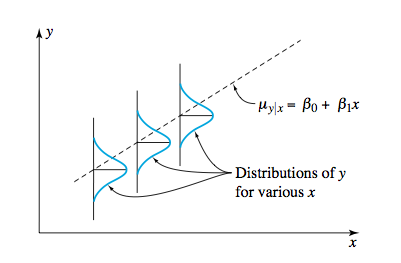
\includegraphics{../../fig/normalsimplereg.png}
\begin{itemize}
\item That's why we do inference.
\end{itemize}
\end{frame}


\begin{frame}
\frametitle{SLR: mean response at $x$}
\begin{itemize}
\item Under the model, $\wh{\mu}_{y \mid x}$ is normally distributed with:
\begin{align*}
\uncover<2->{E(\wh{\mu}_{y \mid x})} &\uncover<2->{= \mu_{y \mid x} =  \beta_0 + \beta_1 x}  \\
\uncover<3->{Var(\wh{\mu}_{y \mid x})} & \uncover<3->{= \sigma^2 \left ( \frac{1}{n} + \frac{(x - \ov{x})^2}{\sum_i(x_i - \ov{x})^2} \right )}
\end{align*}
\uncover<4->{\item We can construct a $N(0,1)$ random variable by standardizing:}
\begin{align*}
\uncover<5->{Z = \frac{\wh{\mu}_{y \mid x} - \mu_{y \mid x}}{  \sigma \sqrt{    \frac{1}{n} \frac{(x - \ov{x})^2}{\sum_i(x_i - \ov{x})^2}   }  } \sim N(0,1)}
\end{align*}
\uncover<6->{\item Replacing $\sigma$ with $s_{LF} = \sqrt{\frac{1}{n-2} \sum_i (y_i - \wh{y}_i)^2}$:}
\begin{align*}
\uncover<7->{T = \frac{\wh{\mu}_{y \mid x} - \mu_{y \mid x}}{  s_{LF} \sqrt{    \frac{1}{n} \frac{(x - \ov{x})^2}{\sum_i(x_i - \ov{x})^2}   }  } \sim t_{n - 2}}
\end{align*}
\end{itemize}
\end{frame}


\begin{frame}
\frametitle{SLR: mean response at $x$} \small
\begin{itemize}
\item To test $H_0: \mu_{y \mid x} = \#$, we can use the test statistic:
\begin{align*}
\uncover<2->{T = \frac{\wh{\mu}_{y \mid x} - \#}{  s_{LF} \sqrt{    \frac{1}{n} +  \frac{(x - \ov{x})^2}{\sum_i(x_i - \ov{x})^2}}}}
\end{align*}
\uncover<3->{which has a $t_{n -2}$ distribution if $H_0$ is true and the model is correct.}
\uncover<4->{\item A 2-sided $1 - \alpha$ confidence interval for $\mu_{y \mid x}$ is:}
\begin{align*}
&\uncover<5->{ \left (\wh{\mu}_{y \mid x} - t_{n - 2, \ 1 - \alpha/2} \cdot  s_{LF} \sqrt{    \frac{1}{n} +  \frac{(x - \ov{x})^2  }{\sum_i(x_i - \ov{x})^2} } , \right . \\ 
& \qquad \left . \wh{\mu}_{y \mid x} + t_{n - 2, \ 1 - \alpha/2} \cdot    s_{LF} \sqrt{    \frac{1}{n} + \frac{(x - \ov{x})^2}{\sum_i(x_i - \ov{x})^2}}  \right )}
\end{align*}
\uncover<6->{and the one-sided intervals are analogous.}
\end{itemize}
\end{frame}

\begin{frame}[fragile]
\frametitle{\small Pressing pressures and specimen densities for a ceramic compound}
\scriptsize
A mixture of $\text{Al}_2\text{O}_3$, polyvinyl alcohol, and water was prepared, dried overnight, crushed, and sieved to obtain 100 mesh size grains. These were pressed into cylinders at pressures from 2,000 psi to 10,000 psi, and cylinder densities were calculated. 

% latex table generated in R 3.5.2 by xtable 1.8-3 package
% Thu Apr 09 12:36:48 2020
\begin{table}[ht]
\centering
\begin{tabular}{rr}
 x (pressure in psi) & y (density in g/cc) \\ 
  \hline
2000.00 & 2.49 \\ 
  2000.00 & 2.48 \\ 
  2000.00 & 2.47 \\ 
  4000.00 & 2.56 \\ 
  4000.00 & 2.57 \\ 
  4000.00 & 2.58 \\ 
  6000.00 & 2.65 \\ 
  6000.00 & 2.66 \\ 
  6000.00 & 2.65 \\ 
  8000.00 & 2.72 \\ 
  8000.00 & 2.77 \\ 
  8000.00 & 2.81 \\ 
  10000.00 & 2.86 \\ 
  10000.00 & 2.88 \\ 
  10000.00 & 2.86 \\ 
  \end{tabular}
\end{table}


\end{frame}


\begin{frame}
\frametitle{Example: ceramics} \small
\begin{itemize}
\item First, I'll make a 2-sided 95\% confidence interval for the true mean density of the ceramics at 4000 psi.
\begin{align*}
\uncover<2->{\wh{\mu}_{y \mid x} = 2.375 + 0.0000487 (4000) = 2.5697 g/cc}
\end{align*}
\uncover<3->{With $ t_{n - 2, \ 1 - \alpha/2}  = t_{13, 0.975} = 2.160$, the margin of error in the confidence interval is:}
\begin{align*}
&\uncover<4->{ t_{n - 2, \ 1 - \alpha/2} \cdot  s_{LF} \sqrt{    \frac{1}{n} +  \frac{(x - \ov{x})^2  }{\sum_i(x_i - \ov{x})^2}}}  \\
 &\uncover<5->{=  2.160(0.0199) \sqrt{\frac{1}{15} + \frac{(4000 - 6000)^2}{1.2 \times 10^8}} = 0.0136 g/cc}
\end{align*}
\uncover<6->{Hence, the $95\%$ CI is:}
\begin{align*}
\uncover<7->{(2.5697 - 0.0136, \ 2.5697 + 0.0136) = (2.5561, \ 2.5833)}
\end{align*}
\uncover<8->{\item We're 95\% confident that the true mean density of the ceramics at 4000 psi is between 2.5561 g/cc and 2.5833 g/cc.}
\end{itemize}
\end{frame}


\begin{frame}
\frametitle{Your turn: ceramics}

\begin{itemize}
\item Calculate and interpret a 2-sided 95\% confidence interval for the true mean density at 5000 psi, given:
\begin{itemize}
\item $\wh{\mu}_{y \mid x} = 2.375 + 0.0000487 x$
\item The margin of error is $t_{n - 2, 1 - \alpha/2} s_{LF} \sqrt{\frac{1}{n} +  \frac{(x - \ov{x})^2  }{\sum_i(x_i - \ov{x})^2}}$
\item $\sum_{i}(x_i - \ov{x})^2 = 1.2 \times 10^8$
\item $n = 15$, $\ov{x} = 6000$.
\item $s_{LF} = 0.0199$
\item $t_{13, 0.975} = 2.16$
\end{itemize}
\item Test $H_0: \beta_0 = 0$ vs. $H_a: \beta_0 \ne 0$ at significance level $\alpha = 0.05$ using the method of p-values.
\end{itemize}
\end{frame}


\begin{frame}<handout:\answers>
\frametitle{Answers: ceramics} \small
\begin{itemize}
\item Make a 2-sided 95\% confidence interval for the true mean density of the ceramics at 5000 psi:
\begin{align*}
\uncover<2->{\wh{\mu}_{y \mid x} = 2.375 + 0.0000487 (5000) = 2.6183 g/cc}
\end{align*}
\uncover<3->{With $ t_{n - 2, \ 1 - \alpha/2}  = t_{13, 0.975} = 2.160$, the margin of error in the confidence interval is:}
\begin{align*}
&\uncover<4->{ t_{n - 2, \ 1 - \alpha/2} \cdot  s_{LF} \sqrt{    \frac{1}{n} +  \frac{(x - \ov{x})^2  }{\sum_i(x_i - \ov{x})^2}}}  \\
 &\uncover<5->{= 2.160(0.0199) \sqrt{\frac{1}{15} + \frac{(5000 - 6000)^2}{1.2 \times 10^8}} = 0.0118 g/cc}
\end{align*}
\uncover<6->{Hence, the $95\%$ CI is:}
\begin{align*}
\uncover<7->{(2.6183 - 0.0118, \ 2.6183 + 0.0118) = (2.6065, \ 2.6301)}
\end{align*}
\uncover<8->{\item We're 95\% confident that the true mean density of the ceramics at 5000 psi is between 2.6065 g/cc and 2.6301 g/cc.}
\end{itemize}
\end{frame}

\begin{frame}<handout:\answers>
\frametitle{Answers: ceramics}
Now for the hypothesis test:
\begin{enumerate}[1. ]
\item $H_0: \beta_0 = 0$, \ $H_a: \beta_0 \ne 0$
\pause \item $\alpha = 0.05$
\pause \item $\beta_0$ is just $\mu_{y \mid x = 0}$. The test statistic is:
\begin{align*}
\uncover<4->{T = \frac{b_0 - 0}{  s_{LF} \sqrt{    \frac{1}{n} +  \frac{(0 - \ov{x})^2}{\sum_i(x_i - \ov{x})^2}}}}  \uncover<5->{= \frac{b_0 }{  s_{LF} \sqrt{    \frac{1}{n} +  \frac{ \ov{x}^2}{\sum_i(x_i - \ov{x})^2}}}}
\end{align*}
\begin{itemize}
\uncover<6->{\item $T \sim t_{n - 2}$ assuming:}
\begin{itemize}
\uncover<7->{\item $H_0$ is true.}
\uncover<8->{\item The model $Y_i = \beta_0 + \beta_1 x_i + \e_i$ is correct, with $\e_1, \ldots \e_n \sim$ iid $N(0,1)$.}
\end{itemize}
\end{itemize}
\end{enumerate}
\end{frame}


\begin{frame}<handout:\answers>
\frametitle{Answers: ceramics}
\begin{enumerate}[1. ]
\setcounter{enumi}{3}
\item The observed test statistic:
\begin{align*}
\uncover<2->{b_0} & \uncover<2->{= 2.375} \\
\uncover<3->{t} & \uncover<3->{= \frac{2.375}{0.0199 \sqrt{ \frac{1}{15} + \frac{6000^2}{1.2 \times 10^8}}}} \uncover<4->{ = 197.09} \\
\uncover<5->{\text{p-value}} &\uncover<5->{= P(|t_{13}| > 197.09) \ll 0.0001}
\end{align*}
\uncover<6->{\item With a p-value $\ll 0.0001 < \alpha$, we reject $H_0$ and conclude $H_a$.}
\uncover<7->{\item There is overwhelming evidence that the intercept of the ``true" line is different from 0.}
\end{enumerate}
\end{frame}

\begin{frame}
\frametitle{Ceramics: back to the JMP output}
\begin{center}
\setkeys{Gin}{width=.48\textwidth} 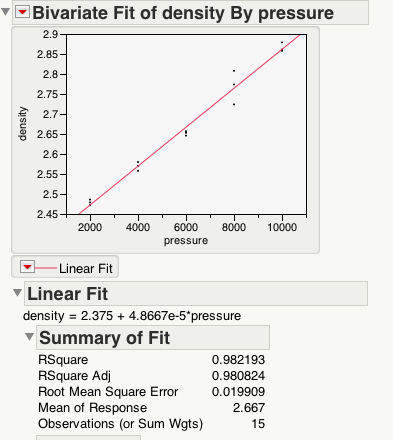
\includegraphics{../../fig/jmpcer1.png}
\setkeys{Gin}{width=.48\textwidth} 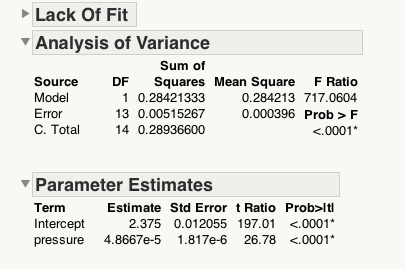
\includegraphics{../../fig/jmpcer2.png}
\end{center}
\end{frame}

\begin{frame}
\frametitle{Ceramics: back to the JMP output}
\begin{center}
\setkeys{Gin}{width=1\textwidth} 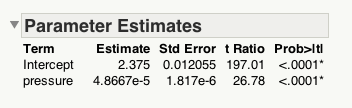
\includegraphics{../../fig/jmpcerparams.png}
\end{center}
\begin{itemize}
\item The observed test statistic $t$ is under ``t Ratio" for the intercept.
\pause \item ``Prob$>|t|$" for the intercept is the p-value for the significance test you just did.
\pause \item ``Estimate" for the intercept is $b_0$.
\pause \item ``Std Error" for the intercept is:
\pause \begin{align*}
\wh{SD}(b_0) = s_{LF} \sqrt{    \frac{1}{n} +  \frac{ \ov{x}^2}{\sum_i(x_i - \ov{x})^2}} 
\end{align*}
\end{itemize}
\end{frame}

\begin{frame}
\frametitle{Be careful with Inference on $\beta_0$}
\begin{itemize}
\item In this case and many others, $\beta_0 = \mu_{y \mid x=0}$ is beyond the range of our data.
\pause \item Estimating beyond the range of our covariate values is called {\bf extrapolation}, which is dangerous for linear regression.
\pause \item Only extrapolate when:
\begin{itemize}
\pause \item You know your process or system well, and can describe it with the right equations.
\pause \item You estimate the parameters of the resulting model using \emph{nonlinear} regression:
\begin{itemize}
\pause \item Example: special case of the Michaelis-Menten model for enzyme kinetics with reaction speed $y$ and substrate concentration $x$:
\pause \begin{align*}
Y_i = \frac{\theta_1 x_i}{ \theta_2 + x_i} + \e_i
\end{align*}
\end{itemize}
\pause \item See \underline{Nonlinear Regression Analysis and Its Applications} by Bates and Watts for more information on nonlinear regression.
\end{itemize}
\end{itemize}
\end{frame}


\section{Prediction interval for a new $y$ at some $x$}
\begin{frame}
\frametitle{Prediction interval for a new $y$ at some $x$} \small
\begin{itemize}
\item The prediction interval in SLR is trying to capture the next response at a given value of predictor variable. 
{\item A 2-sided $1 - \alpha$ prediction interval for a new response $y$ at some $x$ is:}
\begin{align*}
&\uncover<5->{ \left (\wh{\mu}_{y \mid x} - t_{n - 2, \ 1 - \alpha/2} \cdot  s_{LF} \sqrt{1+    \frac{1}{n} +  \frac{(x - \ov{x})^2  }{\sum_i(x_i - \ov{x})^2} } , \right . \\ 
& \qquad \left . \wh{\mu}_{y \mid x} + t_{n - 2, \ 1 - \alpha/2} \cdot    s_{LF} \sqrt{1+    \frac{1}{n} + \frac{(x - \ov{x})^2}{\sum_i(x_i - \ov{x})^2}}  \right )}
\end{align*}
\uncover<6->{and the one-sided intervals are analogous.}
\end{itemize}
\end{frame}



\begin{frame}
\frametitle{Example: ceramics} \small
\begin{itemize}
\item We will make a 2-sided 95\% prediction interval for the next density of the ceramics at 4000 psi.
\begin{align*}
\uncover<2->{\wh{\mu}_{y \mid x} = 2.375 + 0.0000487 (4000) = 2.5697 g/cc}
\end{align*}
\uncover<3->{With $ t_{n - 2, \ 1 - \alpha/2}  = t_{13, 0.975} = 2.160$, the margin of error in the confidence interval is:}
\begin{align*}
&\uncover<4->{ t_{n - 2, \ 1 - \alpha/2} \cdot  s_{LF} \sqrt{  1 +  \frac{1}{n} +  \frac{(x - \ov{x})^2  }{\sum_i(x_i - \ov{x})^2}}}  \\
 &\uncover<5->{=  2.160(0.0199) \sqrt{1 + \frac{1}{15} + \frac{(4000 - 6000)^2}{1.2 \times 10^8}} = 0.0451 g/cc}
\end{align*}
\uncover<6->{Hence, the $95\%$ CI is:}
\begin{align*}
\uncover<7->{(2.5697 - 0.0451, \ 2.5697 + 0.0451) = (2.5246, \ 2.6148)}
\end{align*}
\uncover<8->{\item We're 95\% confident that the next collected density of the ceramics at 4000 psi is between 2.5246 g/cc and 2.6148 g/cc.}
\end{itemize}
\end{frame}

\section{Simultaneous Confidence Intervals for $\mu_{y \mid x}$}

\begin{frame}
\frametitle{Simultaneous confidence intervals}
\begin{itemize}
\item Situations will arise when you'll want to do inference on $\mu_{y \mid x = 2000}, \mu_{y \mid x = 4000}, \mu_{y \mid x = 6000}, \ldots$, all at once.
\pause \item When you compute several confidence intervals at once or do multiple tests at once, you need to account for the simultaneity.
\pause \item On average, for every 20 tests you do independently at $\alpha = 0.05$,  we expect 1 of those tests to conclude $H_a$ by chance alone.
\begin{itemize}
\pause \item Remember: $\alpha$ = P(reject $H_0$ assuming $H_0$ is true).
\end{itemize}
\end{itemize}
\end{frame}


\begin{frame}
\frametitle{Example: \url{http://xkcd.com/882/}}
\setkeys{Gin}{width=1\textwidth} 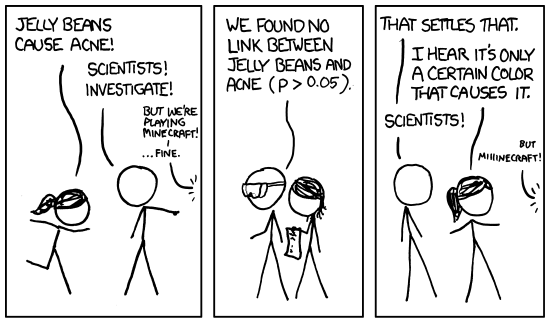
\includegraphics{../../fig/xkcd1.png}
\end{frame}

\begin{frame}
\frametitle{Example: \url{http://xkcd.com/882/}}
\setkeys{Gin}{width=1\textwidth} 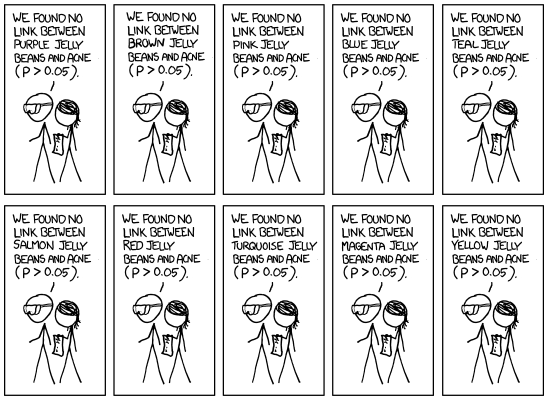
\includegraphics{../../fig/xkcd2.png}
\end{frame}

\begin{frame}
\frametitle{Example: \url{http://xkcd.com/882/}}
\setkeys{Gin}{width=1\textwidth} 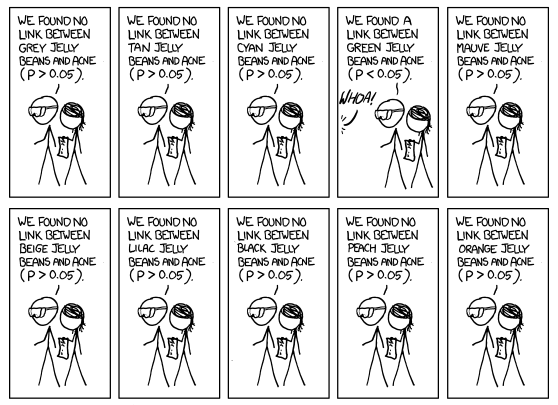
\includegraphics{../../fig/xkcd3.png}
\end{frame}

\begin{frame}
\frametitle{Example: \url{http://xkcd.com/882/}}
\begin{center}
\setkeys{Gin}{width=.7\textwidth} 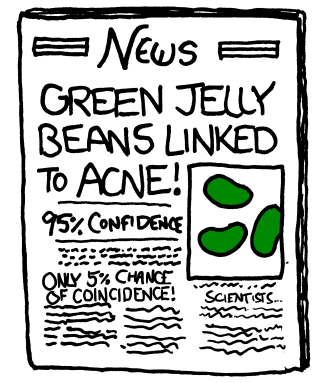
\includegraphics{../../fig/xkcd4.png}
\end{center}
\end{frame}

\begin{frame}
\frametitle{Simultaneous confidence interval}
\scriptsize
\begin{itemize}
\item
If we have $k$ simutaneous tests, each with type I error $\alpha$, then the type I error for the simutaneous tests is
\[P(\mbox{at least one rejection in these $k$ tests}) > \alpha\]
If these tests are independent, the actual type I error is
\begin{align*}
&P(\mbox{at least one rejection in these $k$ tests}) \\
=& 1 - P(\mbox{no rejection in these $k$ tests}) \\
=& 1 - \prod_{i=1}^k P(\mbox{fail to reject the $i$-th test}) = 1 - (1 - \alpha)^k
\end{align*}
\item
For $k$ confidence intervals for $\mu_1, \mu_2, \ldots, \mu_k$, denote the corresponding random intervals $I_1, I_2, \ldots, I_k$. If the confidence level is $1 - \alpha$, then
\[P(\mu_i \in I_i) = 1 - \alpha,\, i = 1, 2, \ldots, k\]
And the simutaneous confidence level would be
\[P(\mbox{$\mu_1 \in I_1$ and $\mu_2 \in I_2$ and $\cdots \mu_k \in I_k$ at the same time} ) < 1 - \alpha\]
\item
To get the $1 - \alpha$ simutaneous confidence level, the simultaneous confidence intervals should be {\bf wider} then individual confidence interval.
\end{itemize}
\end{frame}

\begin{frame}
\frametitle{Simultaneous confidence intervals for $\mu_{y \mid x}$}
\begin{itemize}
\item 
Let $I_x$ be the random intervals for the simultaneous $1 - \alpha$ confidence intervals for $\mu_{y|x}$. Then we want
\[P(\mbox{$\mu_{y|x} \in I_x$ at the same time for all $x$}) = 1 - \alpha\]
\item The simultaneous confidence intervals for $\mu_{y \mid x}$ are given by:
\pause \begin{align*}
b_0 + b_1 x \pm \sqrt{2 F_{2, n-2, 1 - \alpha}} \cdot s_{LF} \cdot \sqrt{ \frac{1}{n} + \frac{(x - \ov{x})^2}{\sum_i(x_i - \ov{x})^2}}
\end{align*}
\pause \item This formula accounts for the fact that we're computing $k$ confidence intervals at the same time.
\end{itemize}
\end{frame}

\begin{frame}
\frametitle{Simultaneous confidence intervals for $\mu_{y \mid x}$}
\setkeys{Gin}{width=.8\textwidth} 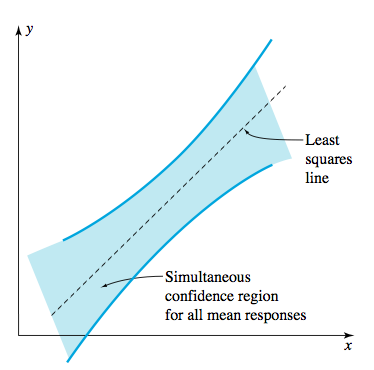
\includegraphics{../../fig/simconf.png}
\end{frame}

\begin{frame}
\frametitle{Example: ceramics}
\begin{itemize}
\item Given:
\begin{itemize}
\pause \item $n = 15$
\pause \item $\ov{x} = 6000$
\pause \item $\sum_i(x_i - \ov{x})^2 = 1.2\times 10^8$
\pause \item $\wh{y} = 2.375 + 4.87 \times 10^{-5} x$, $s_{LF} = 0.0199$.
\pause \item The simultaneous confidence interval formula is:
\pause \begin{align*}
b_0 + b_1 x \pm \sqrt{2 F_{2, k, 1 - \alpha/2}}  \cdot s_{LF} \cdot \sqrt{ \frac{1}{n} + \frac{(x - \ov{x})^2}{\sum_i(x_i - \ov{x})^2}}
\end{align*}
\end{itemize}
\pause \item I will calculate simultaneous 95\% confidence intervals for the mean responses $\mu_{y \mid x}$ at $x = 2000$, 4000, 6000, 8000, and 10000.
\end{itemize}
\end{frame}

\begin{frame}
\frametitle{Example: ceramics} \small
\begin{itemize}
\item Using $F_{2, n-2, 1 - \alpha} = F_{2, 13, 0.95} = 3.81$, the intervals are of the form:
\end{itemize}
\begin{align*}
&\uncover<2->{2.375 + 4.87 \times 10^{-5} x \pm \sqrt{2 \cdot 3.81} \cdot 0.0199 \cdot \sqrt{ \frac{1}{15} + \frac{(x - 6000)^2}{1.2 \times 10^8}}} \\
&\uncover<3->{= 2.375 + 4.87 \times 10^{-5} x \pm 0.0549 \sqrt{0.066 + 8.33 \times 10^{-9} (x - 6000)^2}}
\end{align*}

\begin{center}
\uncover<4->{\begin{tabular}{ccc}
x, pressure & CI, compact form & CI \\ \hline
2000 & $2.4723 \pm 0.0246$ & (2.4477, 2.4969) \\ 
4000 & $2.5697 \pm 0.0174$ & (2.5523, 2.5871) \\ 
6000 & $2.6670 \pm 0.0142$ & (2.6528, 2.6812) \\ 
8000 & $2.7643 \pm 0.0174$ & (2.7469, 2.7817) \\ 
10000 & $2.8617 \pm 0.0246$ & (2.8371, 2.8863) \\ 
\end{tabular}}
\end{center}
\end{frame}


\begin{frame}
\frametitle{Ceramics; plotting simultaneous confidence regions}
\setkeys{Gin}{width=.6\textwidth} 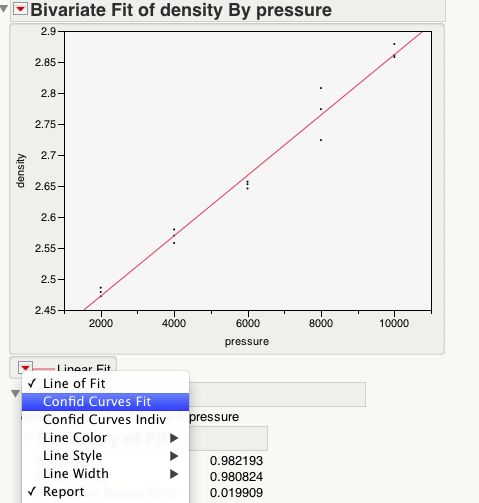
\includegraphics{../../fig/scp1.png}
\end{frame}


\begin{frame}
\frametitle{Ceramics; plotting simultaneous confidence regions}
\setkeys{Gin}{width=.6\textwidth} 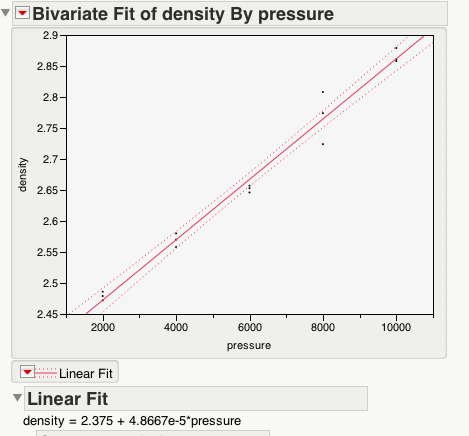
\includegraphics{../../fig/scp2.png}
\end{frame}


\begin{frame}
\frametitle{Ceramics; plotting simultaneous confidence regions}
\setkeys{Gin}{width=.6\textwidth} 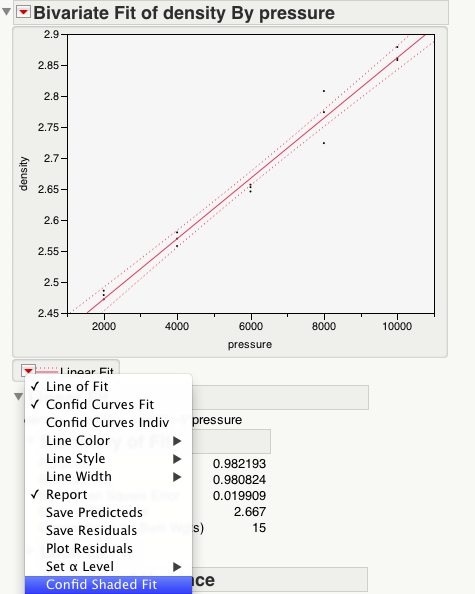
\includegraphics{../../fig/scp3.png}
\end{frame}

\begin{frame}
\frametitle{Ceramics; plotting simultaneous confidence regions}
\setkeys{Gin}{width=.6\textwidth} 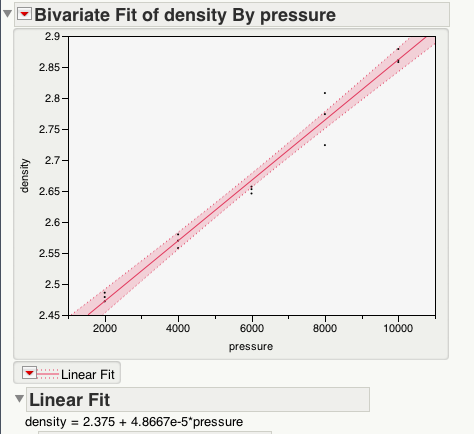
\includegraphics{../../fig/scp4.png}
\end{frame}

\begin{frame}
\frametitle{Ceramics: calculating the margins of error in JMP}
\setkeys{Gin}{width=1\textwidth} 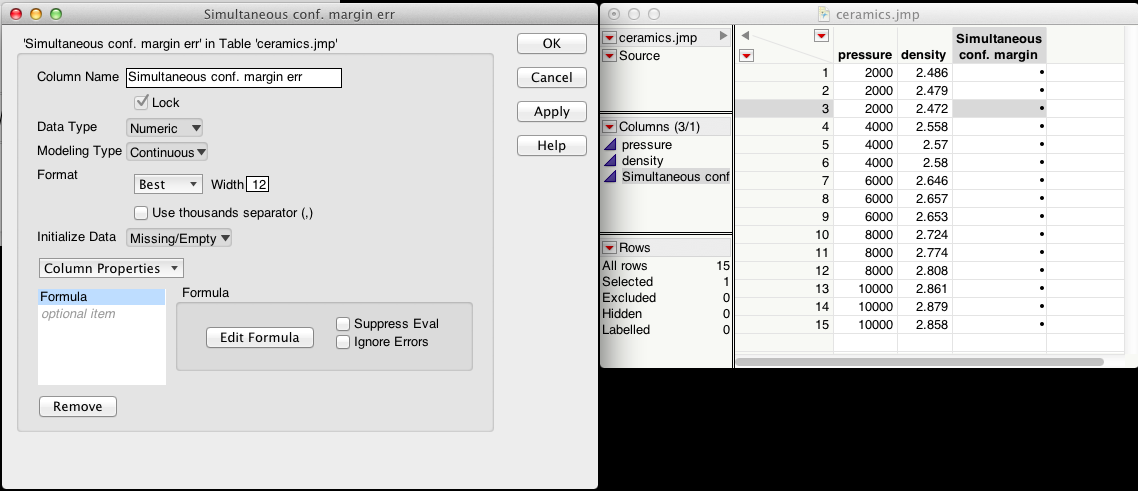
\includegraphics{../../fig/jfs2.png}
\end{frame}

\begin{frame}
\frametitle{Ceramics: calculating the margins of error in JMP}
\setkeys{Gin}{width=.8\textwidth} 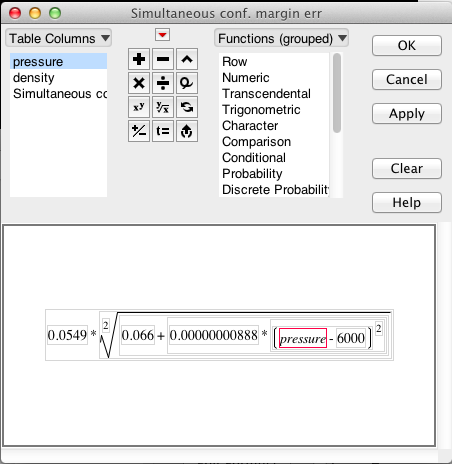
\includegraphics{../../fig/jfs3.png}
\end{frame}

\begin{frame}
\frametitle{Ceramics: calculating the margins of error in JMP}
\setkeys{Gin}{width=1\textwidth} 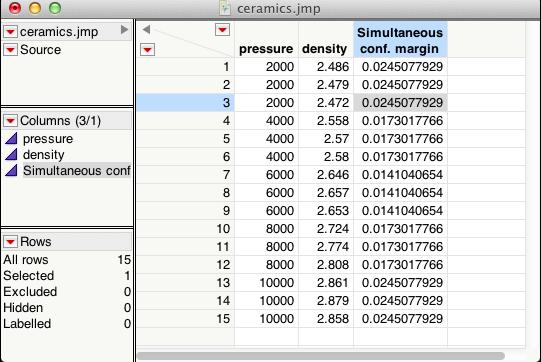
\includegraphics{../../fig/jfs4.png}
\end{frame}

\begin{frame}
\frametitle{Ceramics: calculating the margins of error in JMP}
\setkeys{Gin}{width=1\textwidth} 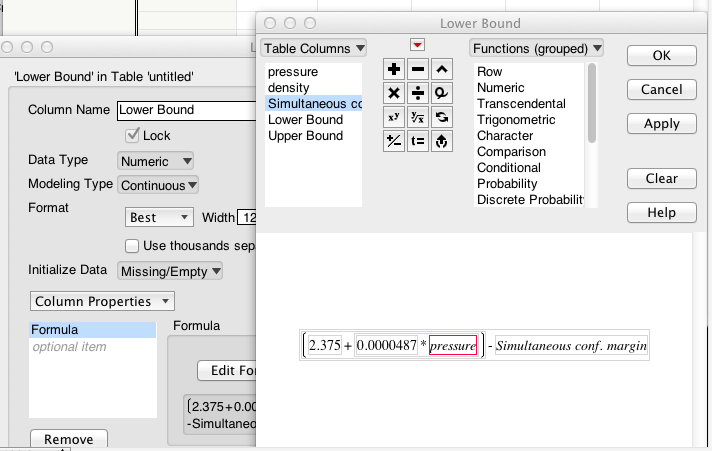
\includegraphics{../../fig/simuljmp11.png}
\end{frame}

\begin{frame}
\frametitle{Ceramics: calculating the margins of error in JMP}
\setkeys{Gin}{width=1\textwidth} 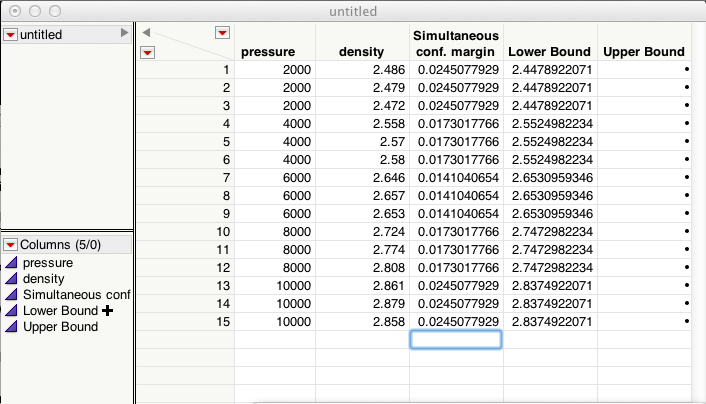
\includegraphics{../../fig/simuljmp12.png}
\end{frame}

\begin{frame}
\frametitle{Ceramics: calculating the margins of error in JMP}
\setkeys{Gin}{width=1\textwidth} 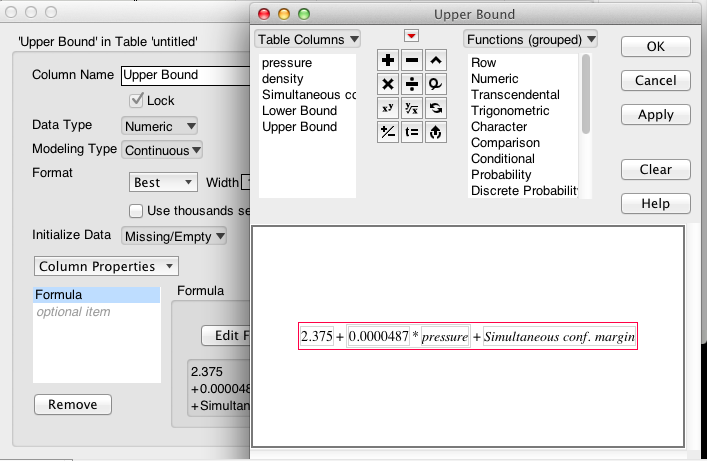
\includegraphics{../../fig/simuljmp21.png}
\end{frame}

\begin{frame}
\frametitle{Ceramics: calculating the margins of error in JMP}
\setkeys{Gin}{width=1\textwidth} 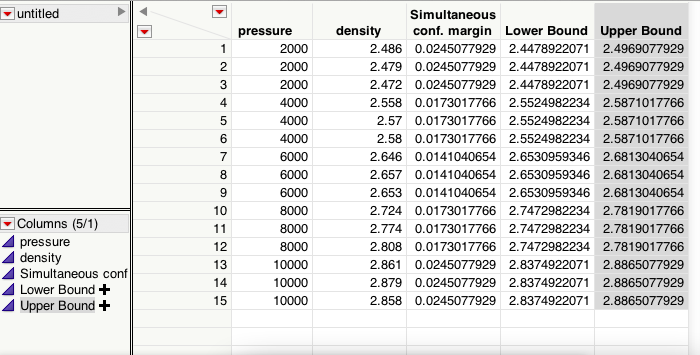
\includegraphics{../../fig/simuljmp22.png}
\end{frame}


\end{document}
